\section{Symmetries}
With the boundary conditions considered, the problem is symmetric about $b/2$. Therefor the problem may be redefined as the left half of the domain, with boundary $\Gamma=\Gamma_1\cup\Gamma_2\cup\Gamma_3\cup\Gamma_4$, see Figure~\ref{fig:domain_new}. \begin{Figure}
 \centering
 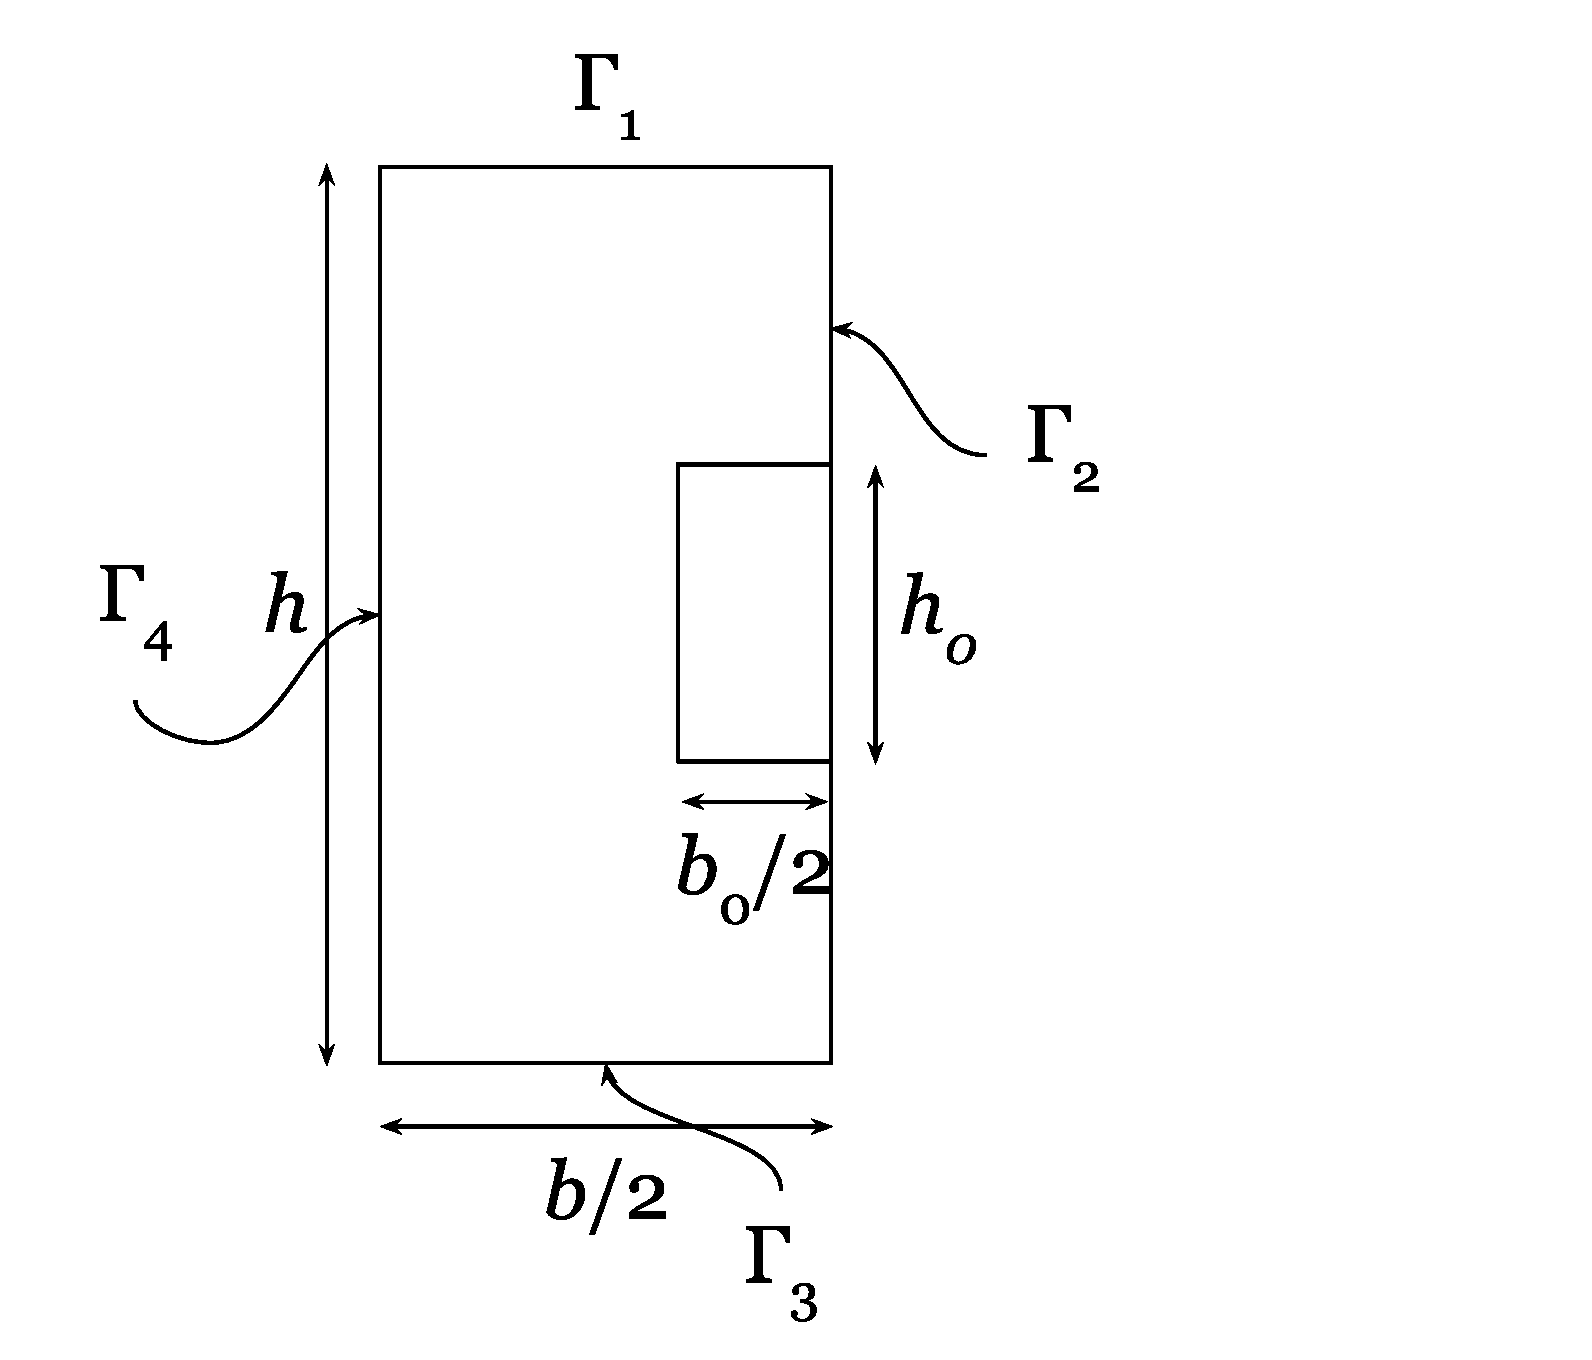
\includegraphics[width=0.7\linewidth]{domain_new.eps}
 \captionof{figure}{Newly defined domain $\Omega$.}\label{fig:domain_new}
\end{Figure} The boundary conditions become:
\begin{equation}
\begin{gathered}
    K\frac{\partial T}{\partial n}\arrowvert_{\Gamma_1\prime} = -\alpha \left(T_w - T_{\infty}\right),\\
    \frac{\partial T}{\partial n}\arrowvert_{\Gamma_2\prime} = 0,\\
    \frac{\partial T}{\partial n}\arrowvert_{\Gamma_3\prime} = 0,\\
    T\arrowvert_{\Gamma_4\prime} = T_0.
\end{gathered}\label{eq:bc}
\end{equation}.


\section{Minimization problem}
To derive the minimization problem for Eq. \ref{eq:heat}, theorem 5.8.1 from Numerical Methods in Scientific Computing \cite{kan}. To use this theorem, homogeneous boundary conditions are needed. Define $v=T-w$, where $w$ satisfies (\ref{eq:bc}). $v$ now satifies homogeneous boundary conditions. The operator in this problem is $L=-k\Delta$, and $L(T)=0$. $L$ needs to be self-adjoint, linear and positive over a space $\Sigma$. Where $\Sigma$ is a vector space consisting of all smooth functions satisfying the homogenous boundary conditions. $L$ is linear if $L(\alpha u+\beta v)=\alpha Lu+\beta Lv, \forall\alpha,\beta\in\mathbb{R}$:
\begin{gather*}
    L(\alpha u+\beta v)\\
    =-\Delta(\alpha u + \beta v)\\
    =-\alpha\Delta u-\beta \Delta v\\
    = \alpha Lu+\beta Lv.
\end{gather*}So L is linear.

Operator $L$ is self-adjoint if $\int\displaylimits_\Omega uLv~\text{d}\Omega=\int\displaylimits_\Omega vLu~\text{d}\Omega, \forall u,v\in~\Sigma$:
\begin{gather*}
    \int\displaylimits_\Omega uLv~\text{d}\Omega = -\int\displaylimits_\Omega u\Delta v~\text{d}\Omega\\
    =-\int\displaylimits_\Omega \nabla \cdot (u\nabla v) - \nabla u\cdot\nabla v~\text{d}\Omega.
\end{gather*}
Using Gau\ss's theorem and the boundary conditions (\ref{eq:bc}):
\begin{gather*}
    =-\int\displaylimits_{\partial\Omega} u\frac{\partial v}{\partial n}~\text{d}\Gamma + \int\displaylimits_\Omega \nabla u\cdot\nabla v~\text{d}\Omega\\
    =\int\displaylimits_\Omega \nabla u\cdot \nabla v\text{d}\Omega
\end{gather*}
The same derivation also holds for $v$ and since $\int\displaylimits_\Omega \nabla u\cdot \nabla v~\text{d}\Omega = \int\displaylimits_\Omega \nabla v\cdot \nabla u~\text{d}\Omega$, $L$ is self-adjoint.

For $L$ to be positive aswell, $\int\displaylimits_\Omega uLu~\text{d}\Omega$ should be greater than or equation to 0, for all $u\in \Sigma$:
\begin{gather*}
    \int\displaylimits_\Omega uLu~\text{d}\Omega = - \int\displaylimits_\Omega u\Delta v~\text{d}\Omega\\
    = -\int\displaylimits_\Omega \nabla \cdot(u\nabla u) - \nabla u\cdot\nabla u~\text{d}\Omega
\end{gather*} Using Gau\ss's theorem and the boundary conditions (\ref{eq:bc}):
\begin{gather*}
    -\int\displaylimits_{\partial\Omega} u\frac{\partial u}{\partial n}~\text{d}\Gamma + \int\displaylimits_{\Omega} |\nabla u|^2~\text{d}\Omega \\
    =\int\displaylimits_\Omega |\nabla u|^2~\text{d}\Omega \geq 0.
\end{gather*} So $L$ is positive.

The minimization problem thus becomes:
\begin{equation}
    \min_{v\in\Sigma} F(v)=\frac{1}{2}\int\displaylimits_{\Omega}vLv~\text{d}\Omega + \int\displaylimits_{\Omega}vLw~\text{d}\Omega.
\end{equation} Since $w$ is unkown, it needs to be removed from the problem.

Subtitude $v=F-w$:
\begin{equation*}
F(T)=\frac{1}{2}\int\displaylimits_\Omega(T-w)(LT+Lw)~\text{d}\Omega.
\end{equation*} $w$ statisfies the boundary conditions, substituting them gives:
\begin{gather*}
    F(T) = \frac{1}{2}\int\displaylimits_{\Omega}(T-w)(-k\nabla (T+w))~\text{d}\Omega\\
    = \frac{1}{2}\int\displaylimits_{\Omega}\nabla\cdot\left[(T-w)\nabla(-k(T+w))\right]~\text{d}\Omega\\
    - \frac{1}{2}\int\displaylimits_{\Omega}\nabla(T-w)\cdot k\nabla(T+w)~\text{d}\Omega,
\end{gather*}using Gau\ss's theorem:
\begin{gather*}
    = -\frac{1}{2}\int\displaylimits_{\partial\Omega}(T-w)k\nabla(T+w)~\text{d}\Omega\\
    + \frac{1}{2}\int\displaylimits_{\Omega}\nabla(T-w)k\nabla(T+w)~\text{d}\Omega\\
    = -\frac{1}{2}\int\displaylimits_{\Omega}\nabla\cdot k\nabla T - \nabla W\cdot k\nabla w~\text{d}\Omega\\
    -\frac{1}{2}\int\displaylimits_{\partial\Omega}(T-w)k\nabla)(T+w)\text{d}\Gamma.
\end{gather*}Sinse the solution is independent of $w$, it can be left out in the first integral.
\begin{gather*}
    = \frac{1}{2}\int\displaylimits_{\Omega}\nabla T\cdot k\nabla T \text{d}\Omega \\
    -\frac{1}{2}\int\displaylimits_{\partial\Omega}(T-w)k\nabla (T+w)\text{d}\Gamma.
\end{gather*}

\section{Interface between the two materials} 

From \ref{eq:final} we have that $T$ minimizes the following function

\begin{gather*}
F(T) = \frac{1}{2}\int_{\Omega}k\left|\nabla\right|^2\mathrm{d}\Omega + \alpha \int_{\Gamma_1}\left(\frac{1}{2}T^2-TT_{\infty}\right)\mathrm{d}\Gamma\\
\rightarrow \left.\frac{\mathrm{d}}{\mathrm{d}t}F(T+tD)\right|_{t=0} = 0, \forall D \in \sum_0\\
\left.\frac{\mathrm{d}}{\mathrm{d}t}F(T+tD)\right|_{t=0} =  \int_{\Omega_A}k_A\nabla D \nabla T \mathrm{d}\Omega\\ + \int_{\Omega_B}k_B\nabla D \nabla T \mathrm{d}\Omega + \alpha \int_{\Gamma_1}\left(DT-DT_{\infty}\right)\mathrm{d}\Gamma\\
= k_a\int_{\Gamma_{A_{outer}}}D\frac{\partial T}{\partial n}\mathrm{d}\Gamma + k_a\int_{\Gamma_{A_{inner}}}D\frac{\partial T}{\partial n}\mathrm{d}\Gamma - k_a\int_{\Omega_A}D\Delta T \mathrm{d}\Omega \\
+ k_b \int_{k_b}D\frac{\partial T}{\partial n}\mathrm{d}\Gamma - k_b\int_{\Omega_B}D\Delta T \mathrm{d}\Omega + \alpha \int_{\Gamma_1}\left(DT-DT_{\infty}\right)\mathrm{d}\Gamma = 0\\
k_a\int_{\Gamma_{A_{outer}}}D\frac{\partial T}{\partial n}\mathrm{d}\Gamma = 0\\
\int_{\Gamma_{A_{inner}}}D\frac{\partial T}{\partial n}\mathrm{d}\Gamma = -\int_{\Gamma_{B}}D\frac{\partial T}{\partial n}\mathrm{d}\Gamma
\end{gather*}
\begin{gather*}
\left(k_a-k_b\right)\int_{\Gamma_{A_{inner}}}D\frac{\partial T}{\partial n}\mathrm{d}\Gamma - k_a\int_{\Omega_A}D\Delta T \mathrm{d}\Omega\\ - k_b\int_{\Omega_B}D\Delta T \mathrm{d}\Omega + \alpha \int_{\Gamma_1}\left(DT-DT_{\infty}\right)\mathrm{d}\Gamma = 0\\
\end{gather*}


The integral over the boundaries of $A$ is just the sum of the inner and outer boundary. The inner boundary of $A$ coincides with the boundary of $B$. Further, if $k_a$ and $k_b$ are known, each of those integrals is completely determined by $D$ and $T$, so 

\begin{gather*}
k_a\int_{\partial_{A_{inner}}}D\frac{\partial T}{\partial n} \mathrm{d}\Gamma = k_b\int_{\partial_{b}}D\frac{\partial T}{\partial n} \mathrm{d}\Gamma
\end{gather*}

Since this must hold for all $D \in \sum$, we get that

\begin{gather*}
\left.k_a\frac{\partial T}{\partial n}\right|_{\partial_{A_{inner}}} = \left.k_b\frac{\partial T}{\partial n}\right|_{\partial B}
\end{gather*}

%Consider the stationary heat equation, and integrate it over a straight line segment perpendicular to the boundary of $A$ and $B$, from $-\epsilon+x$ to $\epsilon+x$, where $x$ is just a general coordinate.
%
%\begin{gather*}
%-\int_{-\epsilon+x}^{\epsilon+x}\nabla \cdot (k\nabla T)\mathrm{d}x' = -\int_{-\epsilon+x}^{\epsilon+x}\frac{\partial}{\partial n}\cdot (k\frac{\partial}{\partial n} T)\mathrm{d}x'\\
%\left. k(x)\frac{\partial}{\partial n} T\right|_{\epsilon+x}-\left. k(x)\frac{\partial}{\partial n} T\right|_{-\epsilon+x} = 0\\
%\lim_{\epsilon \rightarrow 0}\left. k(x)\frac{\partial}{\partial n} T\right|_{\epsilon+x}-\left. k(x)\frac{\partial}{\partial n} T\right|_{-\epsilon+x}\\
%k_a\frac{\partial T}{\partial n}\left_{\partial A} = k_b\frac{\partial T}{\partial n}\left_{\partial B}
%\end{gather*}

\section{Element matrices and vector}
Using Ritz' method: 
\begin{gather*}
    T(x,y) \simeq T_n(x,y)=\sum_{j=1}^n c_j\varphi_j(x,y),\\
    \frac{\partial T_n}{\partial c_i}=\varphi_i(x,y).
\end{gather*} Filling this in to Eq. \ref{eq:final} gives
\begin{gather*}
    F(T)\simeq F(T_n) = \int\displaylimits_{\Omega}\frac{1}{2} k \left|\nabla T_n\right|^2~\text{d}\Omega + \\ \frac{1}{2}\alpha\int\displaylimits_{\Gamma_1}T_n^2-T_nT_{\infty}~\text{d}\Gamma = 0.
\end{gather*} Differentiating with respect to $c_i$ gives
\begin{gather*}
    \frac{\partial F}{\partial c_i} = \int\displaylimits_{\Omega}k\nabla T_n\cdot\nabla\varphi_i~\text{d}\Omega    +\int\displaylimits_{\Gamma_1}T_n\varphi_i-\varphi_iT_{\infty}~\text{d}\Gamma\\
    = \int\displaylimits_{\Omega}k\nabla\left(\sum_{j=1}^n c_j \varphi_j\right)\cdot \nabla \varphi_i~\text{d}\Omega + \\ \alpha\int\displaylimits_{\Gamma_1} \left(\sum_{j=1}^n c_j \varphi_j\right)\varphi_i - \varphi_i T_{\infty}~\text{d}\Gamma,\\
    \sum_{j=1}^n c_j \int\displaylimits_{\Omega}k\nabla\varphi_i\cdot \nabla \varphi_i~\text{d}\Omega \\
    = - \sum_{j=1}^n c_j\left(c_j\alpha\int\displaylimits_{\Gamma_1} \varphi_i \varphi_j~\text{d}\Gamma \right)+\alpha\int\displaylimits_{\Gamma_1}\varphi_i T_{\infty}~\text{d}\Gamma.
\end{gather*} Now the element matrix of an triangular internal element $e_k$ with vertices $\vec{x}_{k_1}$, $\vec{x}_{k_2}$ and $\vec{x}_{k_3}$, becomes
\begin{gather*}
    S_{ij}^{e_k} =  k\int\displaylimits_{e_k} \nabla \varphi_j \cdot \nabla \varphi_j~\text{d}\Omega \\
    = k\left(\beta_i^{e_k} \beta_j^{e_k} \gamma_i^{e_k} \gamma_j^{e_k} \right)\int\displaylimits_{e_k}~\text{d}\Omega.
\end{gather*} Using Holand \& Bell's theorem for the integral, this becomes
\begin{gather}
    S_{ij}^{e_k} = k \frac{|\Delta_{e_k}|}{2}\left(\beta_i^{e_k} \beta_j^{e_k} \gamma_i^{e_k} \gamma_j^{e_k} \right),
\end{gather} where $\frac{|\Delta_{e_k}|}{2}$ is the surface of the element.

The element matrix of a boundary element $be_l$ with vertices $\vec{x}_{l_1}$ and $\vec{x}_{l_2}$, becomes
\begin{gather*}
    S_{ij}^{be_l} = \alpha \int\displaylimits_{be_l}\varphi_i \varphi_j~\text{d}\Gamma,
\end{gather*} using Holand \& Bell's theorem:
\begin{gather}
    S_{ij}^{be_l} = \alpha \frac{\lVert \vec{x}_{l_1} - \vec{x}_{l_2} \rVert}{6} \left( 1 + \delta_{ij} \right).
\end{gather}
The element vector of a boundary element $be_l$, becomes
\begin{gather*}
    \vec{f}_i^{be_l} = \alpha \int\displaylimits_{be_l}\varphi_i T_{\infty}~\text{d}\Gamma = \alpha T_{\infty} \int\displaylimits_{be_l}\varphi_i~\text{d}\Gamma,
\end{gather*} again using Holand \& Bell's theorem:
\begin{gather}
    \vec{f}_i^{be_l} = \alpha T_{\infty} \frac{\lVert \vec{x}_{l_1} - \vec{x}_{l_2} \rVert}{2}.
\end{gather}